\documentclass{article}
\usepackage{fancyhdr}
\usepackage{ctex}
\usepackage{listings}
\usepackage{graphicx}
\usepackage[a4paper, body={18cm,22cm}]{geometry}
\usepackage{amsmath,amssymb,amstext,wasysym,enumerate,graphicx}
\usepackage{float,abstract,booktabs,indentfirst,amsmath}
\usepackage{array}
\usepackage{booktabs}
\usepackage{multirow}
\usepackage{url}
\usepackage{diagbox}
\usepackage{hyperref}
\usepackage{listings}
\renewcommand\arraystretch{1.4}
\usepackage{indentfirst}
\setlength{\parindent}{2em}
\usepackage{enumitem}
\usepackage{accsupp}
\setmonofont{Consolas}
\usepackage{listings}
\usepackage{xcolor}
\usepackage{makecell}
\usepackage{subfigure}
\setCJKmonofont{黑体}
\newcommand\emptyaccsupp[1]{\BeginAccSupp{ActualText={}}#1\EndAccSupp{}}
\newcommand\SQL{\texttt{SQL}}
\renewcommand\tt{\texttt}
\lstset{
    % language = C,
    showstringspaces=false,
    xleftmargin = 3em,xrightmargin = 3em, aboveskip = 1em,
	backgroundcolor = \color{white}, % 背景色
	basicstyle = \small\ttfamily, % 基本样式 + 小号字体
	rulesepcolor= \color{gray}, % 代码块边框颜色
	breaklines = true, % 代码过长则换行
	numbers = left, % 行号在左侧显示
	numberstyle=\emptyaccsupp,
    numbersep = 14pt, 
    keywordstyle=\color{purple}\bfseries, % 关键字颜色
    commentstyle =\color{red!50!green!50!blue!60}, % 注释颜色
    stringstyle = \color{red}, % 字符串颜色
    morekeywords={ASSERT, int64_t, uint32_t},
	% frame = shadowbox, % 用(带影子效果)方框框住代码块
	frame = single, % 用(带影子效果)方框框住代码块
	showspaces = false, % 不显示空格
	columns = fixed, % 字间距固定
  framesep=1em
} 
\lstset{
    sensitive=true,
    moreemph={ASSERT, NULL}, emphstyle=\color{red}\bfseries,
    moreemph=[2]{int64_t, uint32_t, tid_t, uint8_t, int16_t, uint16_t, int32_t, size_t}, emphstyle=[2]\color{purple}\bfseries,
    showspaces = false, % 不显示空格
    }
%--------------------页眉--------------------%
\pagestyle{fancy}
\fancyhead[L]{}
\fancyhead[R]{}
\fancyhead[C]{《数据库系统及应用实践》课程实验报告}
\fancyfoot[C]{-\thepage-}
\renewcommand{\headrulewidth}{1.5pt}
%--------------------标题--------------------%
\begin{document}
\begin{center}
  \LARGE{{\textbf{\heiti 《数据库系统及应用实践》课程实验报告}}}

  \vspace{0.5em}

  \large 实验4:JDBC数据库应用
  \begin{table}[H]
    \centering
    \begin{tabular}{p{2cm}p{2cm}<{\centering}p{0.4cm}p{2cm}p{3cm}<{\centering}p{0.4cm}p{2cm}p{3cm}<{\centering}}
      姓\qquad 名: & 李鹏达 & \quad & 学\qquad 号: & 10225101460 & \quad & 完成日期: & 2024年5月11日 \\ \cline{2-2} \cline{5-5} \cline{8-8}
    \end{tabular}
  \end{table}
\end{center}
% \rule{\textwidth}{1pt}
%--------------------正文--------------------%
\section{实验目标}
\begin{enumerate}[noitemsep]
  \item 学习通过JDBC接口访问关系数据库的基本方法;
  \item 能够根据要求编写程序通过JDBC接口访问关系数据库管理系统;
\end{enumerate}

\section{实验过程记录}

\subsection{安装和配置MySQL的JDBC驱动}

\subsubsection{获取Connector/J 8.3}


MySQL provides connectivity for client applications developed in the Java programming
language with MySQL Connector/J. Connector/J implements the Java Database Connectivity
(JDBC) API, as well as a number of value-adding extensions of it.

实验所用操作系统为 \tt{Ubuntu 24.04 LTS on Windows 10 x86\_64(Kernel: 5.15.146.1-microsoft-\\standard-WSL2)},使用以下命令来安装MySQL的JDBC驱动:

\begin{lstlisting}[language=bash]
wget https://dev.mysql.com/get/Downloads/Connector-J/mysql-connector-j_8.4.0-1ubuntu24.04_all.deb
sudo dpkg -i mysql-connector-j_8.4.0-1ubuntu24.04_all.deb
\end{lstlisting}

安装过程如下图所示:

\begin{figure}[H]
  \centering
  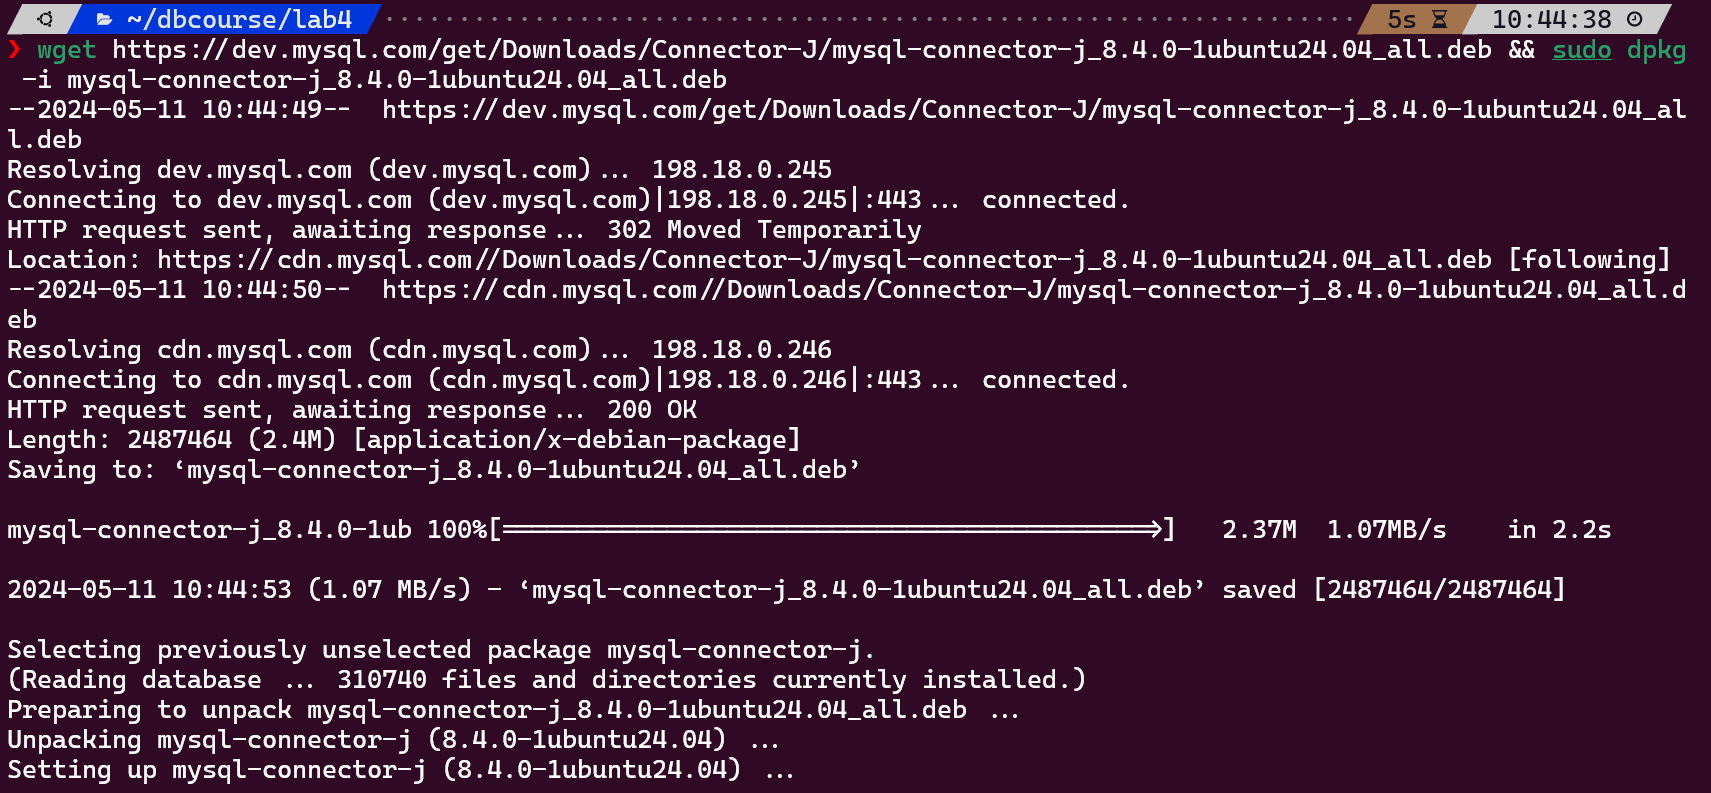
\includegraphics[width=0.66\textwidth]{img/1.png}
  \caption{安装MySQL的JDBC驱动}
\end{figure}

\subsubsection{安装JAVA开发环境}

在这里,我们选择安装 \texttt{openjdk-21},使用以下命令来安装:

\begin{lstlisting}[language=bash]
sudo apt install openjdk-21-jdk
\end{lstlisting}

安装过程如下图所示:

\begin{figure}[H]
  \centering
  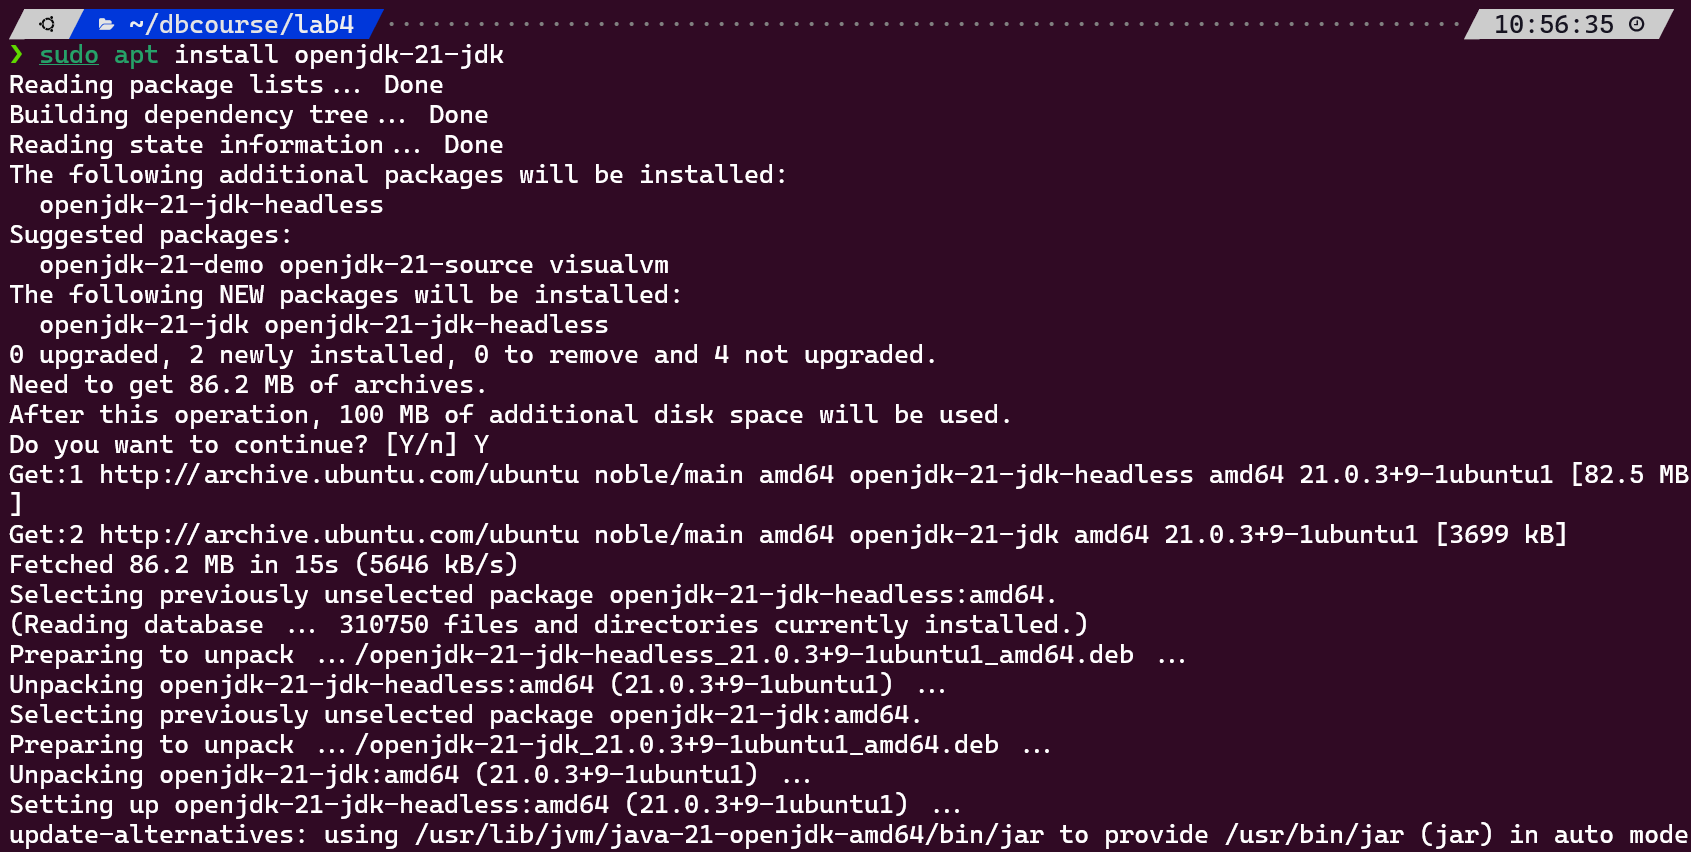
\includegraphics[width=0.9\textwidth]{img/2.png}
  \caption{安装JAVA开发环境}
\end{figure}

\subsubsection{配置环境变量}

我们使用以下命令来配置环境变量(在这里,我是用的shell是 \tt{zsh}):

\begin{lstlisting}[language=bash]
echo 'export JAVA_HOME=/usr/lib/jvm/java-21-openjdk-amd64\nexport PATH=$PATH:$JAVA_HOME/bin\nexport CLASSPATH=$CLASSPATH:/usr/share/java/*:.' >> ~/.zshrc
source ~/.zshrc
\end{lstlisting}

配置过程如下图所示:

\begin{figure}[H]
  \centering
  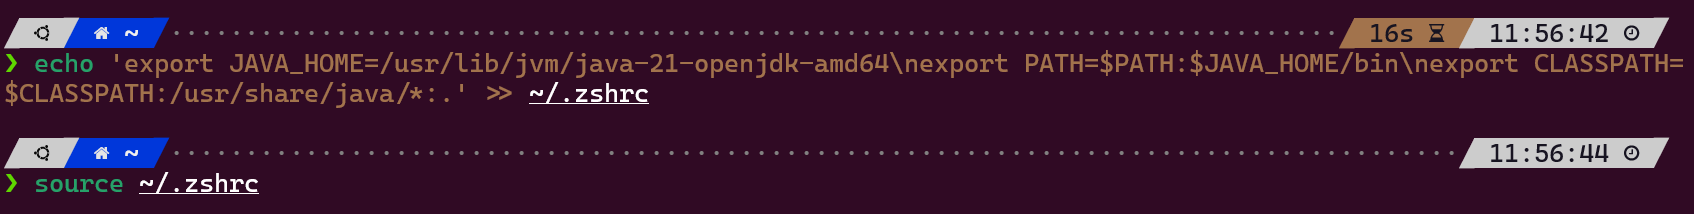
\includegraphics[width=0.9\textwidth]{img/3.png}
  \caption{配置环境变量}
\end{figure}

使用以下命令来检查系统中java的编译和运行环境:

\begin{lstlisting}[language=bash]
javac --version
java --version
\end{lstlisting}

结果如下图所示:

\begin{figure}[H]
  \centering
  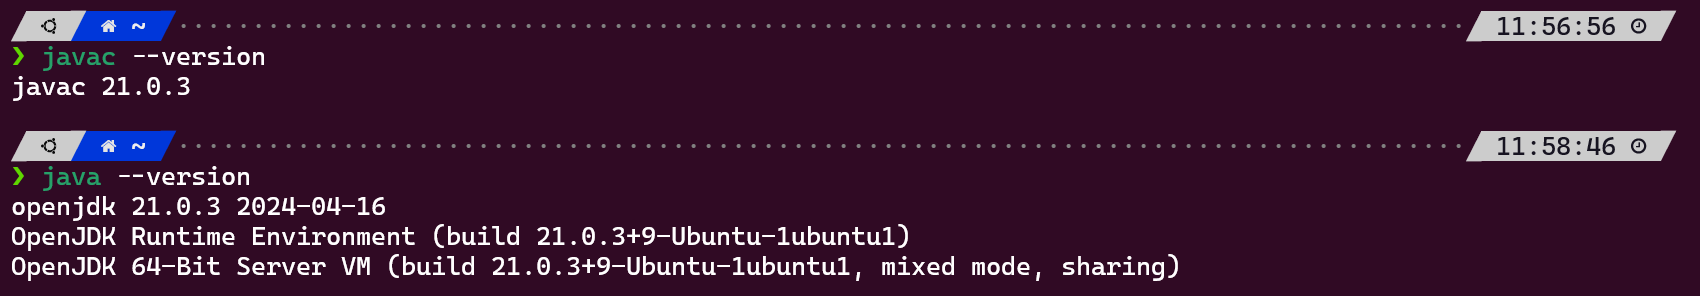
\includegraphics[width=0.9\textwidth]{img/4.png}
  \caption{检查系统中java的编译和运行环境}
\end{figure}

\subsection{JDBC基本操作}

\subsubsection{与数据库建立连接}

在当前工作文件夹中创建一个名为 \tt{jdbcConnect.java} 的文件,其中内容如下:

\begin{lstlisting}[language=java]
import java.sql.Connection;
import java.sql.DriverManager;

public class jdbcConnect {
    public static void main(String args[]) {
        String dbUserName = "root";
        String dbPassword = "password";
        String dbUrl = "jdbc:mysql://localhost:53306/dbcourse?useSSL=false&allowPublicKeyRetrieval=true";
        Connection c = null;
        try {
            Class.forName("com.mysql.cj.jdbc.Driver");
            c = DriverManager.getConnection(dbUrl, dbUserName, dbPassword);
        } catch (Exception e) {
            e.printStackTrace();
            System.err.println(e.getClass().getName() + ": " + e.getMessage());
            System.exit(0);
        }
        System.out.println("Connect to the MySQL database successfully !");
    }
}
  \end{lstlisting}

接下来,使用以下命令来编译和运行该程序:

\begin{lstlisting}[language=bash]
javac jdbcConnect.java && java jdbcConnect
\end{lstlisting}

运行结果如下图所示:

\begin{figure}[H]
  \centering
  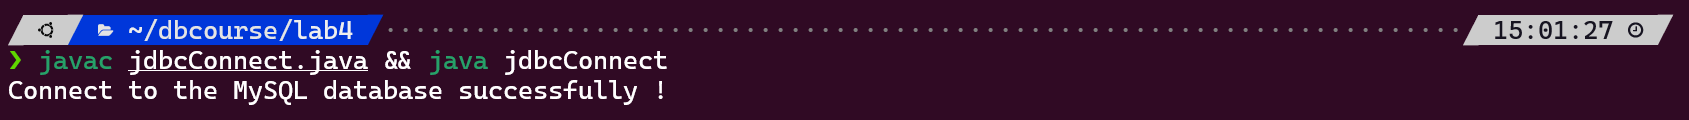
\includegraphics[width=0.9\textwidth]{img/5.png}
  \caption{与数据库建立连接}
\end{figure}

\subsubsection{在数据库中创建数据表}

在当前工作文件夹中创建一个名为 \tt{jdbcCreate.java} 的文件,其中内容如下:

\begin{lstlisting}[language=java]
import java.sql.Connection;
import java.sql.DriverManager;
import java.sql.Statement;

public class jdbcCreate {
    public static void main(String args[]) {
        String dbUserName = "root";
        String dbPassword = "password";
        String dbUrl = "jdbc:mysql://localhost:53306/dbcourse?useSSL=false&allowPublicKeyRetrieval=true";
        Connection c = null;
        Statement stmt = null;
        try {
            Class.forName("com.mysql.cj.jdbc.Driver");
            c = DriverManager.getConnection(dbUrl, dbUserName, dbPassword);
            System.out.println("Connect to the MySQL database successfully!");
            stmt = c.createStatement();
            String sql = """
                    CREATE TABLE employee (
                        id INT,
                        name VARCHAR(20) NOT NULL,
                        age INT NOT NULL,
                        address VARCHAR(50),
                        salary REAL,
                        PRIMARY KEY (id)
                    )
                    """;
            stmt.executeUpdate(sql);
            stmt.close();
            c.close();
        } catch (Exception e) {
            System.err.println(e.getClass().getName() + ": " + e.getMessage());
            System.exit(0);
        }
        System.out.println("Create table employee successfully !");
    }
}
\end{lstlisting}

使用以下命令来编译和运行该程序:

\begin{lstlisting}[language=bash]
javac jdbcCreate.java && java jdbcCreate
\end{lstlisting}

运行结果如下图所示:

\begin{figure}[H]
  \centering
  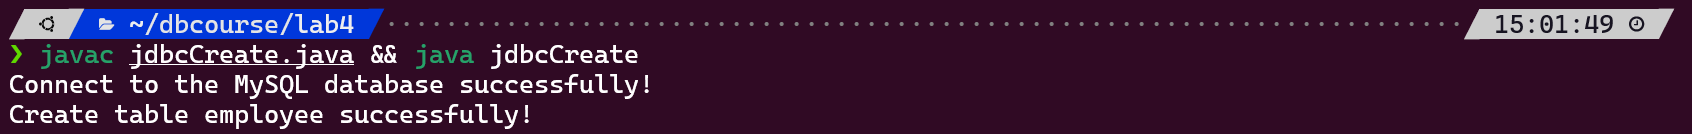
\includegraphics[width=0.9\textwidth]{img/6.png}
  \caption{在数据库中创建数据表}
\end{figure}

\subsubsection{向数据表中插入数据}

在当前工作文件夹中创建一个名为 \tt{jdbcInsert.java} 的文件,其中内容如下:

\begin{lstlisting}[language=java]
import java.sql.Connection;
import java.sql.DriverManager;
import java.sql.Statement;

public class jdbcInsert {
    public static void main(String args[]) {
        String dbUserName = "root";
        String dbPassword = "password";
        String dbUrl = "jdbc:mysql://localhost:53306/dbcourse?useSSL=false&allowPublicKeyRetrieval=true";
        Connection c = null;
        Statement stmt = null;
        try {
            Class.forName("com.mysql.cj.jdbc.Driver");
            c = DriverManager.getConnection(dbUrl, dbUserName, dbPassword);
            c.setAutoCommit(false);
            System.out.println("Connect to the MySQL database successfully!");
            stmt = c.createStatement();
            String sql = "INSERT INTO employee VALUES " +
                    "(1, 'Zhang', 30, '2075 Kongjiang Road', 20000.00 );";
            stmt.executeUpdate(sql);
            sql = "INSERT INTO employee VALUES " +
                    "(2, 'Luan', 25, '3663 Zhongshan Road(N)', 15000.00 );";
            stmt.executeUpdate(sql);
            sql = "INSERT INTO employee VALUES " +
                    "(3, 'Hu', 23, '1234 Beijing Road(E)', 14000.00);";
            stmt.executeUpdate(sql);
            sql = "INSERT INTO employee VALUES " +
                    "(4, 'Jin', 24, '666 Nanjing Road(W)', 19000.00);";
            stmt.executeUpdate(sql);
            sql = "INSERT INTO employee VALUES " +
                    "(5, 'Yi', 24, '100 Renmin Road', 18800.00 );";
            stmt.executeUpdate(sql);
            stmt.close();
            c.commit();
            c.close();
        } catch (Exception e) {
            System.err.println(e.getClass().getName() + ": " + e.getMessage());
            System.exit(0);
        }
        System.out.println("5 records inserted successfully !");
    }
}
\end{lstlisting}

使用以下命令来编译和运行该程序:

\begin{lstlisting}[language=bash]
javac jdbcInsert.java && java jdbcInsert
\end{lstlisting}

运行结果如下图所示:

\begin{figure}[H]
  \centering
  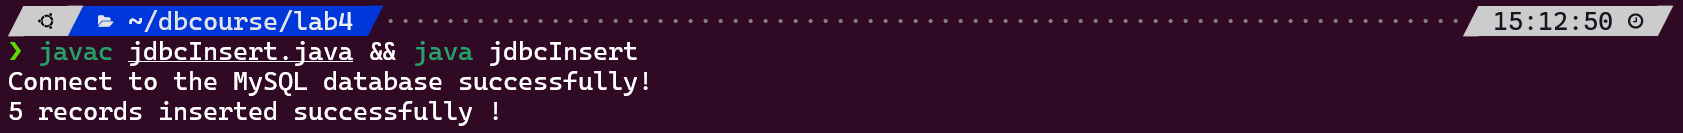
\includegraphics[width=0.9\textwidth]{img/7.png}
  \caption{向数据表中插入数据}
\end{figure}

\subsubsection{从数据表中查询数据}

在当前工作文件夹中创建一个名为 \tt{jdbcSelect.java} 的文件,其中内容如下:

\begin{lstlisting}[language=java]
import java.sql.Connection;
import java.sql.DriverManager;
import java.sql.ResultSet;
import java.sql.Statement;

public class jdbcSelect {
    public static void main(String args[]) {
        String dbUserName = "root";
        String dbPassword = "password";
        String dbUrl = "jdbc:mysql://localhost:53306/dbcourse?useSSL=false&allowPublicKeyRetrieval=true";
        Connection c = null;
        Statement stmt = null;
        try {
            Class.forName("com.mysql.cj.jdbc.Driver");
            c = DriverManager.getConnection(dbUrl, dbUserName, dbPassword);
            c.setAutoCommit(false);
            System.out.println("Connect to the MySQL database successfully!");
            stmt = c.createStatement();
            ResultSet rs = stmt.executeQuery("SELECT * FROM employee;");
            while (rs.next()) {
                int id = rs.getInt("id");
                String name = rs.getString("name");
                int age = rs.getInt("age");
                String address = rs.getString("address");
                float salary = rs.getFloat("salary");
                System.out.println("ID = " + id);
                System.out.println("NAME = " + name);
                System.out.println("AGE = " + age);
                System.out.println("ADDRESS = " + address);
                System.out.println("SALARY = " + salary);
                System.out.println();
            }
            rs.close();
            stmt.close();
            c.close();
        } catch (Exception e) {
            System.err.println(e.getClass().getName() + ": " + e.getMessage());
            System.exit(0);
        }
        System.out.println("Operation done successfully !");
    }
}
\end{lstlisting}

使用以下命令来编译和运行该程序:

\begin{lstlisting}[language=bash]
javac jdbcSelect.java && java jdbcSelect
\end{lstlisting}

运行结果如下图所示:

\begin{figure}[H]
  \centering
  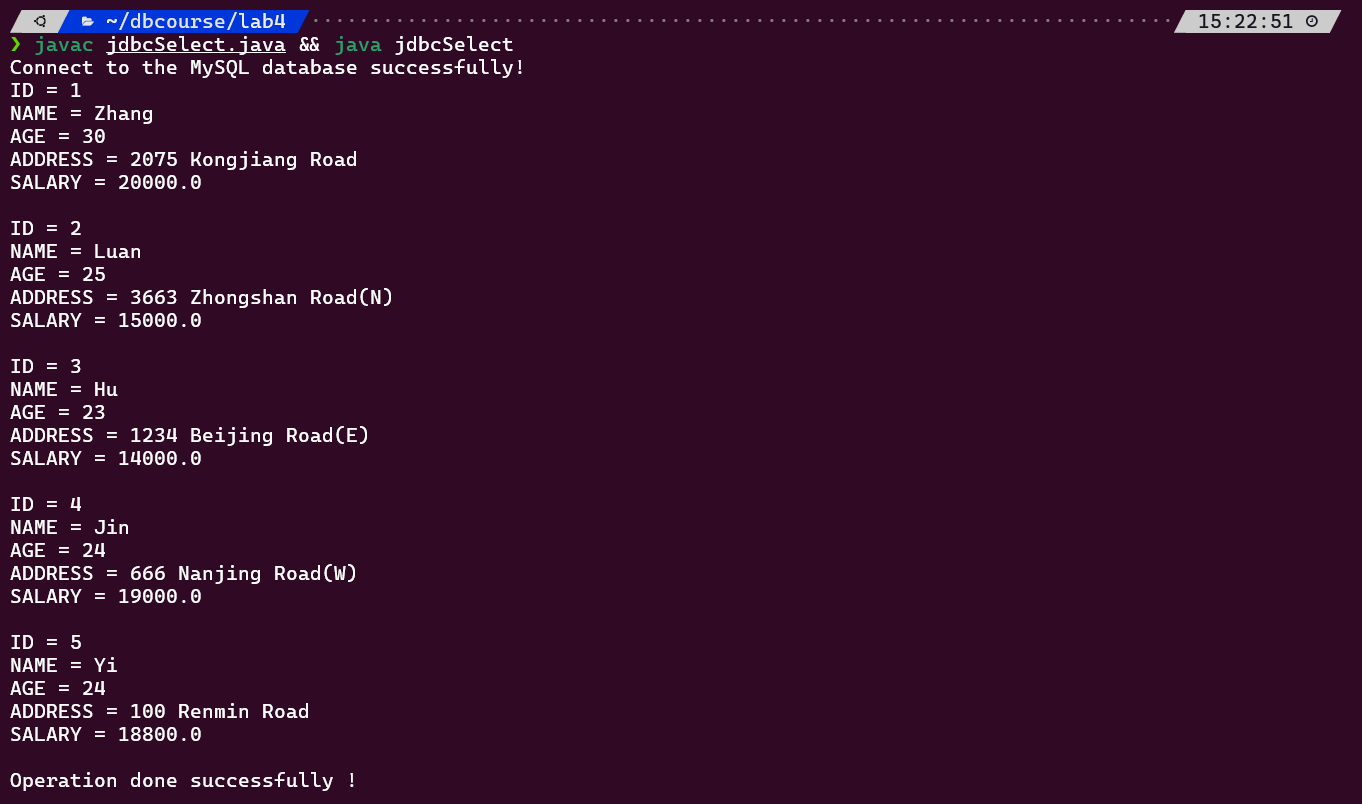
\includegraphics[width=0.9\textwidth]{img/8.png}
  \caption{从数据表中查询数据}
\end{figure}

\subsubsection{更新数据表中的数据}

在当前工作文件夹中创建一个名为 \tt{jdbcUpdate.java} 的文件,其中内容如下:

\begin{lstlisting}[language=java]
import java.sql.Connection;
import java.sql.DriverManager;
import java.sql.ResultSet;
import java.sql.Statement;

public class jdbcUpdate {
    public static void main(String args[]) {
        String dbUserName = "root";
        String dbPassword = "password";
        String dbUrl = "jdbc:mysql://localhost:53306/dbcourse?useSSL=false&allowPublicKeyRetrieval=true";
        Connection c = null;
        Statement stmt = null;
        try {
            Class.forName("com.mysql.cj.jdbc.Driver");
            c = DriverManager.getConnection(dbUrl, dbUserName, dbPassword);
            c.setAutoCommit(false);
            System.out.println("Connect to the MySQL database successfully!");
            stmt = c.createStatement();
            String sql = "UPDATE employee set SALARY = 32000.00 where ID = 1;";
            stmt.executeUpdate(sql);
            c.commit();
            System.out.println("1 record is updated successfully");
            ResultSet rs = stmt.executeQuery("SELECT * FROM employee;");
            while (rs.next()) {
                int id = rs.getInt("id");
                String name = rs.getString("name");
                int age = rs.getInt("age");
                String address = rs.getString("address");
                float salary = rs.getFloat("salary");
                System.out.println("ID = " + id);
                System.out.println("NAME = " + name);
                System.out.println("AGE = " + age);
                System.out.println("ADDRESS = " + address);
                System.out.println("SALARY = " + salary);
                System.out.println();
            }
            rs.close();
            stmt.close();
            c.close();
        } catch (Exception e) {
            System.err.println(e.getClass().getName() + ": " + e.getMessage());
            System.exit(0);
        }
        System.out.println("Operation done successfully !");
    }
}
\end{lstlisting}

使用以下命令来编译和运行该程序:

\begin{lstlisting}[language=bash]
javac jdbcUpdate.java && java jdbcUpdate
\end{lstlisting}

运行结果如下图所示:

\begin{figure}[H]
  \centering
  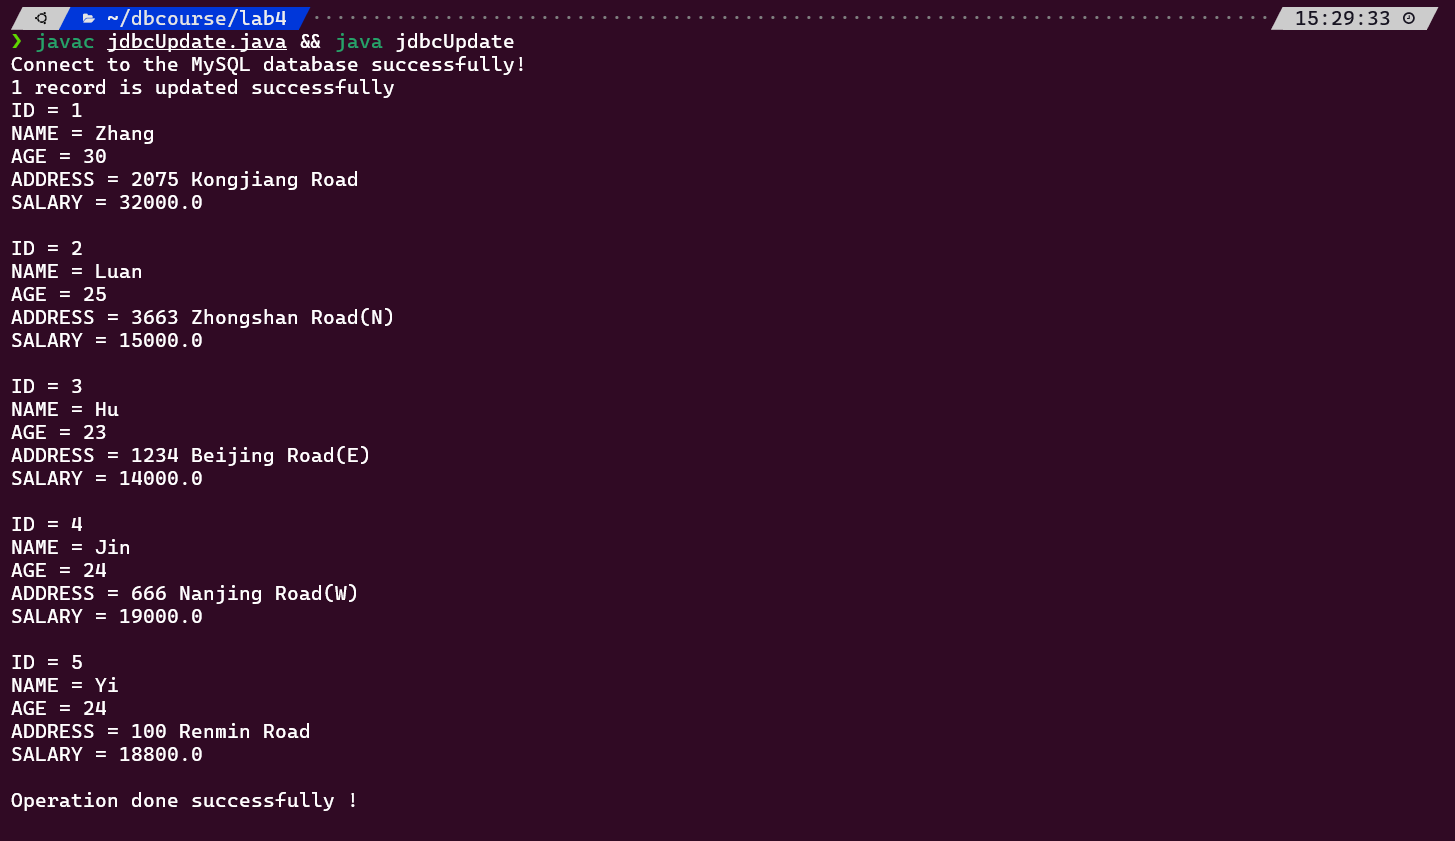
\includegraphics[width=0.9\textwidth]{img/9.png}
  \caption{更新数据表中的数据}
\end{figure}

\subsubsection{删除数据表中的数据}

在当前工作文件夹中创建一个名为 \tt{jdbcDelete.java} 的文件,其中内容如下:

\begin{lstlisting}[language=java]
import java.sql.Connection;
import java.sql.DriverManager;
import java.sql.ResultSet;
import java.sql.Statement;

public class jdbcDelete {
    public static void main(String args[]) {
        String dbUserName = "root";
        String dbPassword = "password";
        String dbUrl = "jdbc:mysql://localhost:53306/dbcourse?useSSL=false&allowPublicKeyRetrieval=true";
        Connection c = null;
        Statement stmt = null;
        try {
            Class.forName("com.mysql.cj.jdbc.Driver");
            c = DriverManager.getConnection(dbUrl, dbUserName, dbPassword);
            c.setAutoCommit(false);
            System.out.println("Connect to the MySQL database successfully!");
            stmt = c.createStatement();
            String sql = "DELETE from employee where ID=2;";
            stmt.executeUpdate(sql);
            c.commit();
            System.out.println("1 record is deleted successfully !");
            ResultSet rs = stmt.executeQuery("SELECT * FROM employee;");
            while (rs.next()) {
                int id = rs.getInt("id");
                String name = rs.getString("name");
                int age = rs.getInt("age");
                String address = rs.getString("address");
                float salary = rs.getFloat("salary");
                System.out.println("ID = " + id);
                System.out.println("NAME = " + name);
                System.out.println("AGE = " + age);
                System.out.println("ADDRESS = " + address);
                System.out.println("SALARY = " + salary);
                System.out.println();
            }
            rs.close();
            stmt.close();
            c.close();
        } catch (Exception e) {
            System.err.println(e.getClass().getName() + ": " + e.getMessage());
            System.exit(0);
        }
        System.out.println("Operation done successfully !");
    }
}
\end{lstlisting}

使用以下命令来编译和运行该程序:

\begin{lstlisting}[language=bash]
javac jdbcDelete.java && java jdbcDelete
\end{lstlisting}

运行结果如下图所示:

\begin{figure}[H]
  \centering
  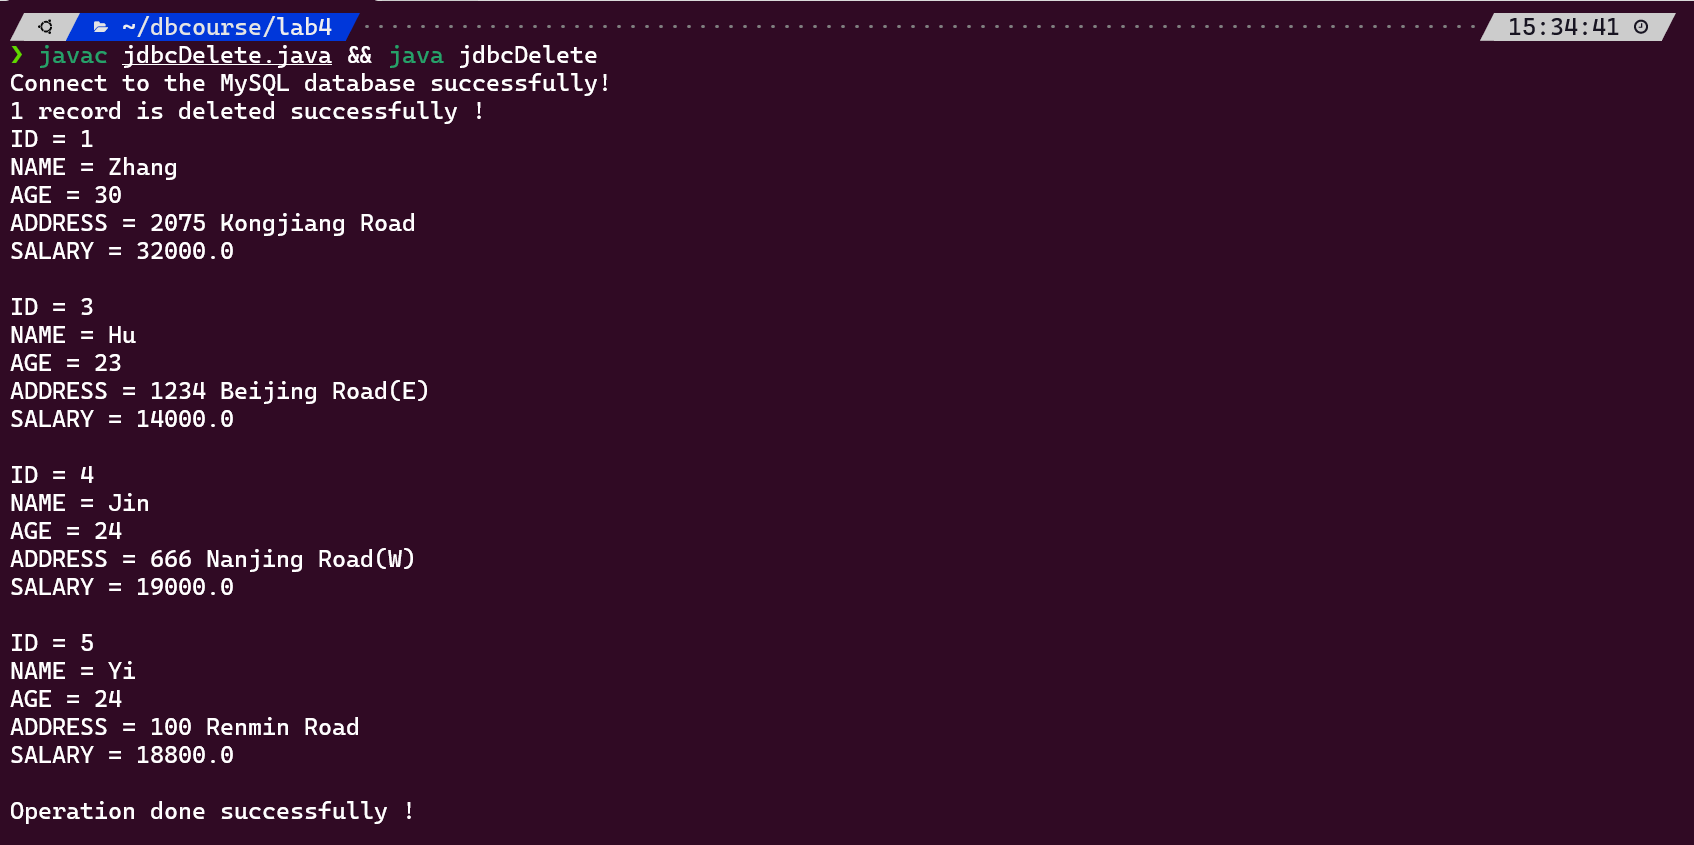
\includegraphics[width=0.9\textwidth]{img/10.png}
  \caption{删除数据表中的数据}
\end{figure}

\subsubsection{使用 prepare 语句向数据表中批量插入(更新)数据}

在当前工作文件夹中创建一个名为 \tt{DBTest.java} 的文件,其中内容如下:

\begin{lstlisting}[language=java]
import java.sql.Connection;
import java.sql.DriverManager;
import java.sql.SQLException;
import java.sql.Statement;
import java.sql.PreparedStatement;

public class DBTest {
    // Connect to database
    public static Connection GetConnection(String username, String passwd) {
        String driver = "com.mysql.cj.jdbc.Driver";
        String sourceURL = "jdbc:mysql://localhost:53306/dbcourse?useSSL=false&allowPublicKeyRetrieval=true";
        Connection conn = null;
        try {
            Class.forName(driver);
            conn = DriverManager.getConnection(sourceURL, username, passwd);
            System.out.println("Connect to database successfully!");
        } catch (Exception e) {
            e.printStackTrace();
            return null;
        }
        return conn;
    };

    // Create table customer
    public static void CreateTable(Connection conn) {
        Statement stmt = null;
        try {
            stmt = conn.createStatement();
            int rc = stmt.executeUpdate("CREATE TABLE customer" +
                    "(id INTEGER, name VARCHAR(20), PRIMARY KEY(id));");
            System.out.println("Create table customer successfully!");
            stmt.close();
        } catch (SQLException e) {
            if (stmt != null) {
                try {
                    stmt.close();
                } catch (SQLException e1) {
                    e1.printStackTrace();
                }
            }
            e.printStackTrace();
        }
    }

    // Execute prepare statement, batch insert
    public static void BatchInsertData(Connection conn) {
        PreparedStatement pst = null;
        try {
            pst = conn.prepareStatement("INSERT INTO customer VALUES (?,?)");
            for (int i = 0; i < 10; i++) {
                pst.setInt(1, i);
                pst.setString(2, "ECNUer " + i);
                pst.addBatch();
            }
            pst.executeBatch();
            System.out.println("Insert 10 record in 1 batch successfully!");
            pst.close();
        } catch (SQLException e) {
            if (pst != null) {
                try {
                    pst.close();
                } catch (SQLException e1) {
                    e1.printStackTrace();
                }
            }
            e.printStackTrace();
        }
    }

    // Update by prepare statement
    public static void ExecPreparedSQL(Connection conn) {
        PreparedStatement pstmt = null;
        try {
            pstmt = conn
                    .prepareStatement("UPDATE customer SET name = ? WHERE id = 1");
            pstmt.setString(1, "Wang");
            int rowcount = pstmt.executeUpdate();
            System.out.println("Update custormer 1's name successfully!");
            pstmt.close();
        } catch (SQLException e) {
            if (pstmt != null) {
                try {
                    pstmt.close();
                } catch (SQLException e1) {
                    e1.printStackTrace();
                }
            }
            e.printStackTrace();
        }
    }

    /**
     * Main program
     */
    public static void main(String[] args) {
        Connection conn = GetConnection("root", "password");
        CreateTable(conn);
        BatchInsertData(conn);
        ExecPreparedSQL(conn);
        try {
            conn.close();
        } catch (SQLException e) {
            e.printStackTrace();
        }
    }
}
\end{lstlisting}

使用以下命令来编译和运行该程序:

\begin{lstlisting}[language=bash]
javac DBTest.java && java DBTest
\end{lstlisting}

运行结果如下图所示:

\begin{figure}[H]
  \centering
  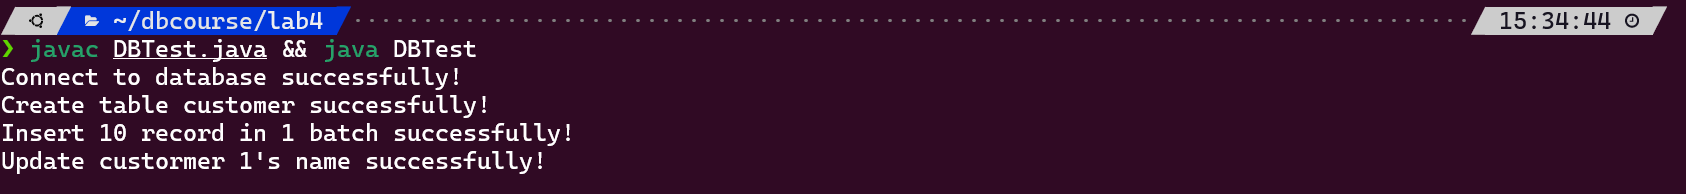
\includegraphics[width=0.9\textwidth]{img/11.png}
  \caption{使用 prepare 语句向数据表中批量插入(更新)数据}
\end{figure}

\subsection{JDBC应用}

\subsubsection{Teaching Record Management System}
Write a Java program that allows university administrators to print the teaching record of an instructor.

\begin{enumerate}[label=(\alph*)]
  \item Start by having the user input the login \textbf{ID} and \textbf{password}; then open the proper connection.
  \item The user is asked next for a search substring and the system returns \tt{(ID, name)} pairs of instructors whose names match the substring. Use the like \tt{('\%substring\%')} construct in SQL to do this. If the search comes back empty, allow continued searches until there is a nonempty result.
  \item Then the user is asked to enter an \textbf{ID} number, which is a number between 0 and 99999. Once a valid number is entered, check if an instructor with that ID exists. If there is no instructor with the given ID, print a reasonable message and quit.
  \item If the instructor has taught no courses, print a message saying that. Otherwise, print the teaching record for the instructor, showing the \textbf{department name, course identifier, course title, section number, semester, year, and total enrollment} (and sort those by dept name, course id, year, semester).
\end{enumerate}

Test carefully for bad input. Make sure your SQL queries won’t throw an exception. At login, exceptions may occur since the user might type a bad password, but catch those exceptions and allow the user to try again.

所写的Java程序如下:

\begin{lstlisting}[language=java]
import java.sql.Connection;
import java.sql.DriverManager;
import java.sql.PreparedStatement;
import java.sql.ResultSet;
import java.sql.SQLException;
import java.util.Scanner;

public class InstructorSystem {
    public static final String url = "jdbc:mysql://localhost:53306/dbcourse?useSSL=false&allowPublicKeyRetrieval=true";

    public static Connection c;

    public static Scanner sc = new Scanner(System.in);

    public static final String spliter = "----------------------------------------";

    public static void login() {
        try {
            String id, password;
            System.out.print("Enter your ID: ");
            id = sc.nextLine();
            System.out.print("Enter your password: ");
            password = sc.nextLine();
            Class.forName("com.mysql.cj.jdbc.Driver");
            c = DriverManager.getConnection(url, id, password);
        } catch (SQLException e) {
            System.out.println("Invalid ID or password! Please try again!");
            login();
        } catch (Exception e) {
            e.printStackTrace();
            System.err.println(
                    "Something went wrong! Please contact the administrator for help or try again later!(check the error message above)");
            System.exit(1);
        }
    }

    public static void searchInstructors() {
        String searchString;
        try {
            System.out.print("Enter the name of the instructor you want to search for: ");
            searchString = sc.nextLine();
            PreparedStatement ps = c.prepareStatement("SELECT `ID`, `name` FROM `instructor` WHERE `name` LIKE ?");
            ps.setString(1, "%" + searchString + "%");
            ResultSet rs = ps.executeQuery();
            if (!rs.isBeforeFirst()) {
                System.out.println("No instructor found! Please try again!");
                searchInstructors();
            }
            System.out.println("Search results:");
            System.out.println(spliter);
            while (rs.next()) {
                System.out.println("ID: " + rs.getInt("id"));
                System.out.println("Name: " + rs.getString("name"));
                System.out.println(spliter);
            }
            rs.close();
            ps.close();
        } catch (Exception e) {
            e.printStackTrace();
            System.err.println(
                    "Something went wrong! Please contact the administrator for help or try again later!(check the error message above)");
            System.exit(1);
        }
    }

    public static Integer checkInstructor() {
        Integer id = null;
        try {
            System.out.print("Enter the ID of the instructor you select: ");
            id = sc.nextInt();
            PreparedStatement ps = c.prepareStatement("SELECT `ID`, `name` FROM `instructor` WHERE `ID` = ?");
            ps.setInt(1, id);
            ResultSet rs = ps.executeQuery();
            if (!rs.isBeforeFirst()) {
                System.out.println("No instructor found! Quitting...");
                System.exit(0);
            }
            rs.close();
            ps.close();
        } catch (SQLException e) {
            e.printStackTrace();
            System.err.println(
                    "Something went wrong! Please contact the administrator for help or try again later!(check the error message above)");
            System.exit(1);
        }
        return id;
    }

    public static void searchTeachingRecords(int id) {
        try {
            PreparedStatement ps = c.prepareStatement(
                """
                SELECT `course`.`dept_name`, `course`.`course_id`, `course`.`title`,
                `section`.`sec_id`, `section`.`semester`, `section`.`year`,
                COUNT(`takes`.`ID`) AS `total_enrollment`
                FROM `teaches` JOIN `course` ON `teaches`.`course_id` = `course`.`course_id`
                JOIN `section` ON `teaches`.`course_id` = `section`.`course_id` AND `teaches`.`sec_id` = `section`.`sec_id`
                LEFT JOIN `takes` ON `teaches`.`course_id` = `takes`.`course_id` AND `teaches`.`sec_id` = `takes`.`sec_id`
                WHERE `teaches`.`ID` = ?
                GROUP BY `course_id`, `sec_id`, `semester`, `year`
                ORDER BY `dept_name`, `course_id`, `year`, `semester`""");
            ps.setInt(1, id);
            ResultSet rs = ps.executeQuery();
            if (!rs.isBeforeFirst()) {
                System.out.println("No teaching record found! Quitting...");
                System.exit(0);
            }
            System.out.println("Teaching records for instructor with ID " + id + ":");
            System.out.println(spliter);
            while (rs.next()) {
                System.out.println("Department: " + rs.getString("dept_name"));
                System.out.println("Course ID: " + rs.getString("course_id"));
                System.out.println("Title: " + rs.getString("title"));
                System.out.println("Section ID: " + rs.getString("sec_id"));
                System.out.println("Semester: " + rs.getString("semester"));
                System.out.println("Year: " + rs.getInt("year"));
                System.out.println("Total Enrollment: " + rs.getInt("total_enrollment"));
                System.out.println(spliter);
            }
        } catch (Exception e) {
            e.printStackTrace();
            System.err.println(
                    "Something went wrong! Please contact the administrator for help or try again later!(check the error message above)");
            System.exit(1);
        }
    }

    public static void main(String[] args) {
        login();
        searchInstructors();
        int instructorID = checkInstructor();
        searchTeachingRecords(instructorID);
    }
}
\end{lstlisting}

使用以下命令来编译和运行该程序:

\begin{lstlisting}[language=bash]
javac InstructorSystem.java && java InstructorSystem
\end{lstlisting}

运行结果如下图所示:


\begin{figure}[htbp]
  \centering
  \begin{subfigure}
    \centering
    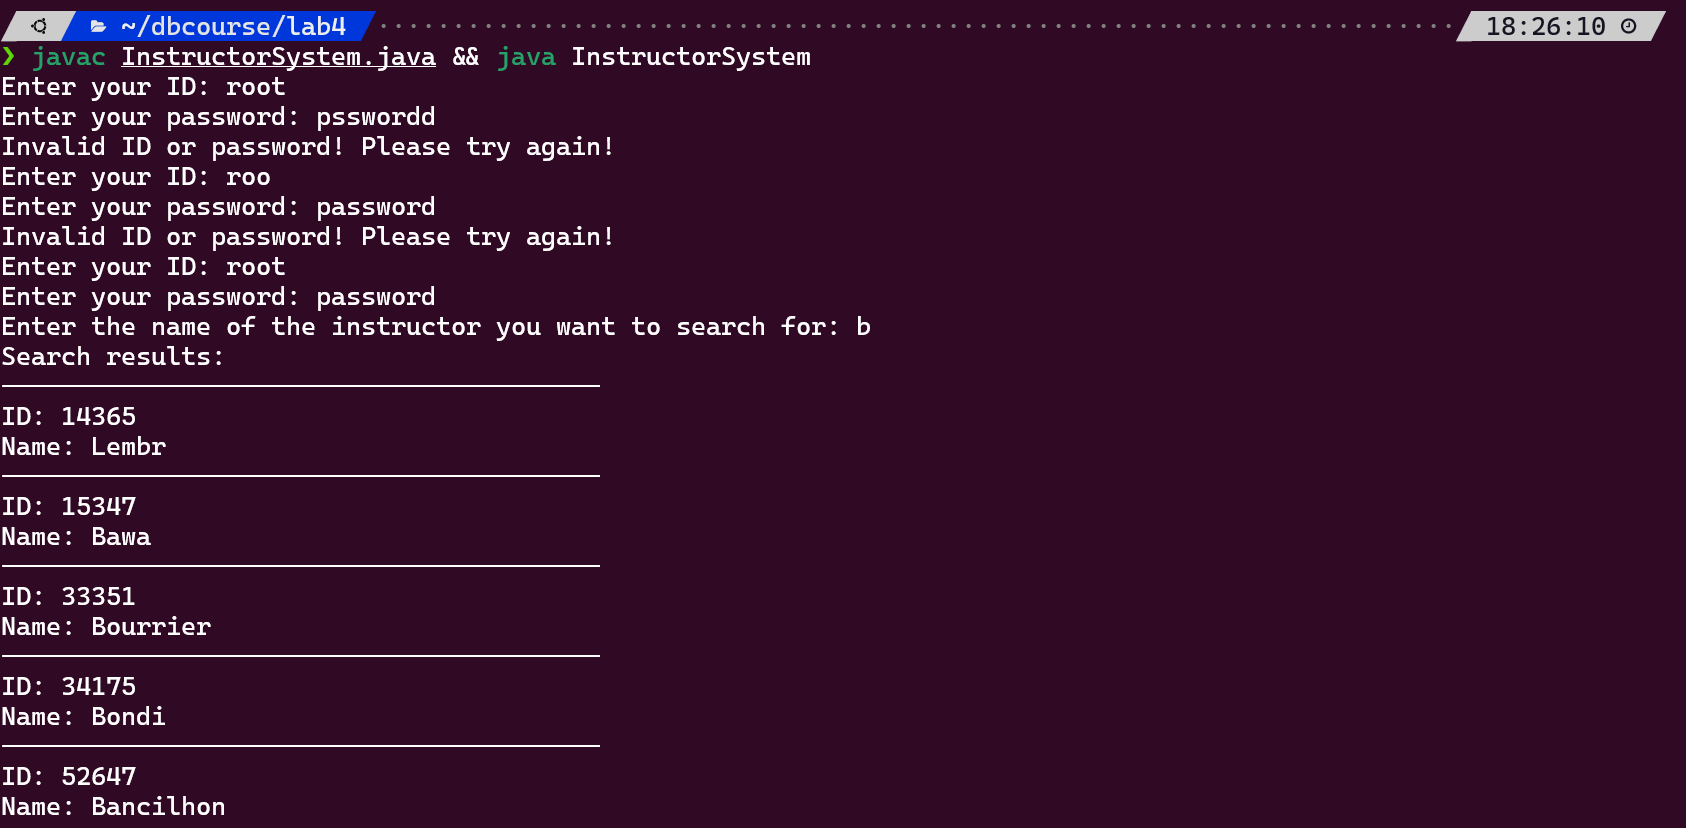
\includegraphics[width=0.76\textwidth]{img/12.png}
  \end{subfigure}
  \hfill
  \begin{subfigure}
    \centering
    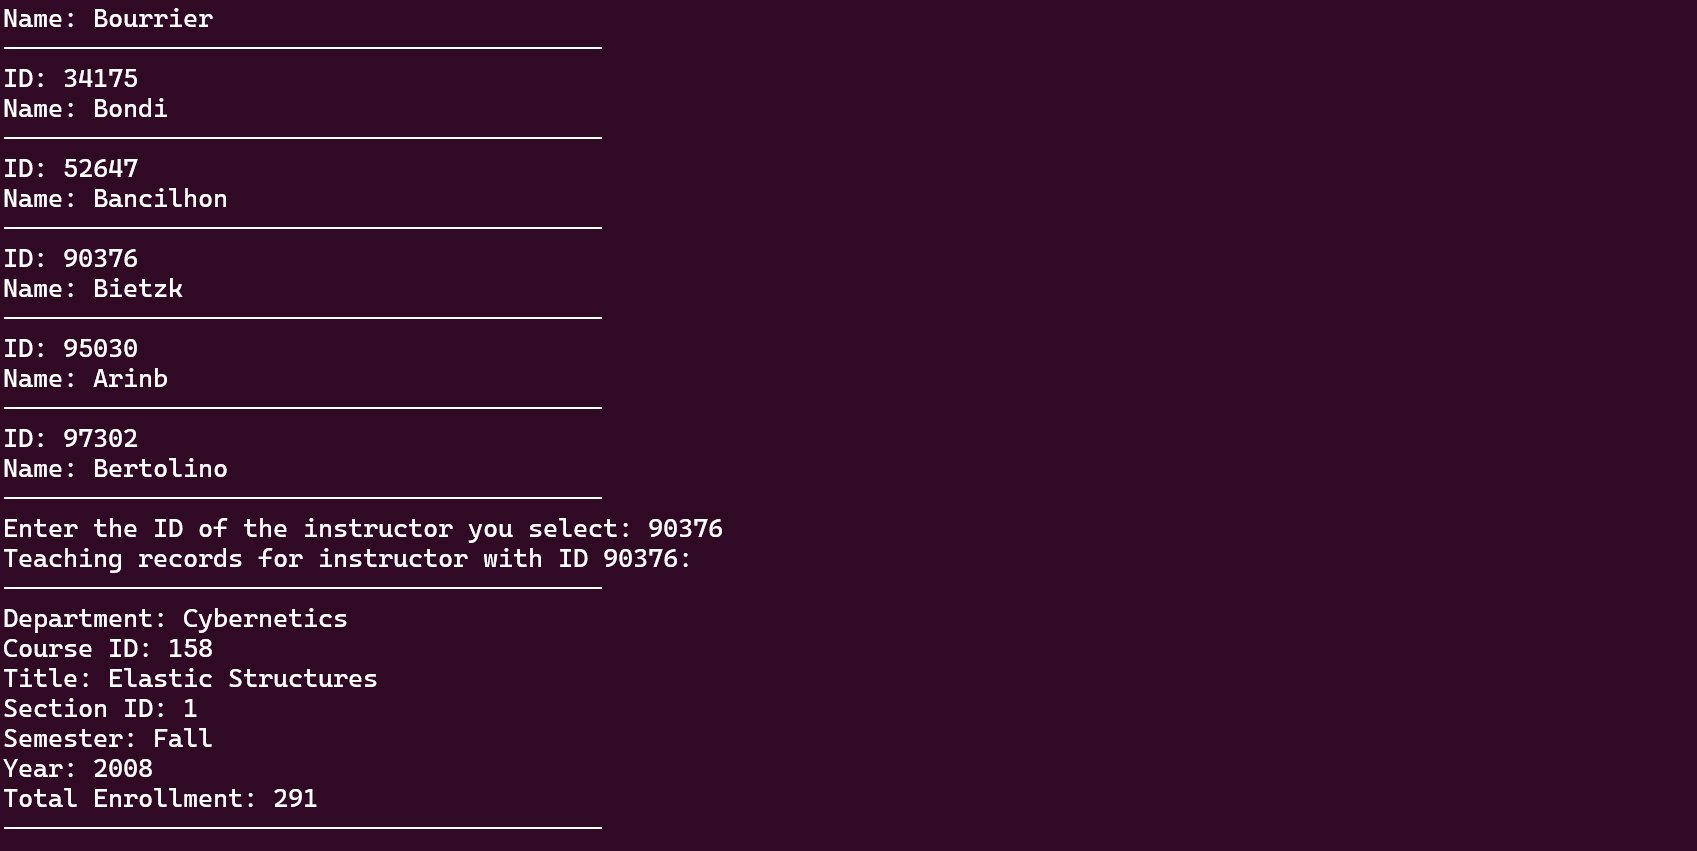
\includegraphics[width=0.76\textwidth]{img/13.png}
  \end{subfigure}
  \caption{Teaching Record Management System}
\end{figure}

\subsection{MetaDisplay}

Suppose you were asked to define a class \tt{MetaDisplay} in Java, containing a method
\begin{center}
  \tt{static void printTable(String r);}
\end{center}

the method takes a relation name \tt{r} as input, executes the query \tt{select * from r}, and
prints the result out in tabular format, with the attribute names displayed in the header of the table.

\begin{enumerate}[label=(\alph*)]
  \item What do you need to know about relation \tt{r} to be able to print the result in the specified tabular format?
  
  我们需要知道关系 \tt{r} 的属性名和属性类型,以便能够正确地打印出表格。
  \item What JDBC methods(s) can get you the required information?
  
  我们可以使用 \tt{ResultSetMetaData} 类的 \tt{getColumnCount()} 和 \tt{getColumnName()} 方法来获取关系 \tt{r} 的属性名。
  \item Write the method \tt{printTable(String r)} using the JDBC API.
\end{enumerate}

所写的Java程序如下:

\begin{lstlisting}[language=java]
import java.sql.Connection;
import java.sql.DriverManager;
import java.sql.ResultSet;
import java.sql.ResultSetMetaData;
import java.sql.SQLException;
import java.sql.Statement;

public class MetaDisplay {
    public static void printTable(String r) {
        String url = "jdbc:mysql://localhost:53306/dbcourse?useSSL=false&allowPublicKeyRetrieval=true";
        String username = "root";
        String password = "password";

        String query = "SELECT * FROM " + r;

        try (Connection connection = DriverManager.getConnection(url, username, password);
                Statement statement = connection.createStatement(ResultSet.TYPE_SCROLL_INSENSITIVE,
                        ResultSet.CONCUR_READ_ONLY);
                ResultSet resultSet = statement.executeQuery(query)) {

            ResultSetMetaData metaData = resultSet.getMetaData();
            int columnCount = metaData.getColumnCount();

            int[] columnWidths = new int[columnCount + 1];

            while (resultSet.next()) {
                for (int i = 1; i <= columnCount; i++) {
                    String columnValue = resultSet.getString(i);
                    if (columnValue == null) {
                        columnValue = "NULL";
                    }
                    columnWidths[i] = Math.max(columnValue.length(), columnWidths[i]);
                }
            }

            resultSet.beforeFirst();

            for (int i = 1; i <= columnCount; i++) {
                System.out.print("+" + "-".repeat(columnWidths[i] + 2));
            }
            System.out.println("+");

            for (int i = 1; i <= columnCount; i++) {
                String columnName = metaData.getColumnName(i);
                System.out.printf("| %" + columnWidths[i] + "s ", columnName);
            }
            System.out.println("|");

            for (int i = 1; i <= columnCount; i++) {
                System.out.print("+" + "-".repeat(columnWidths[i] + 2));
            }
            System.out.println("+");

            while (resultSet.next()) {
                for (int i = 1; i <= columnCount; i++) {
                    String columnValue = resultSet.getString(i);
                    if (columnValue == null) {
                        columnValue = "NULL";
                    }
                    System.out.printf("| %" + columnWidths[i] + "s ", columnValue);
                }
                System.out.println("|");
            }
            for (int i = 1; i <= columnCount; i++) {
                System.out.print("+" + "-".repeat(columnWidths[i] + 2));
            }
            System.out.println("+");

        } catch (SQLException e) {
            e.printStackTrace();
        }
    }

    public static void main(String[] args) {
        printTable("instructor");
    }
}
\end{lstlisting}

使用以下命令来编译和运行该程序:

\begin{lstlisting}[language=bash]
javac MetaDisplay.java && java MetaDisplay
\end{lstlisting}

运行结果如下图所示:

\begin{figure}[H]
  \centering
  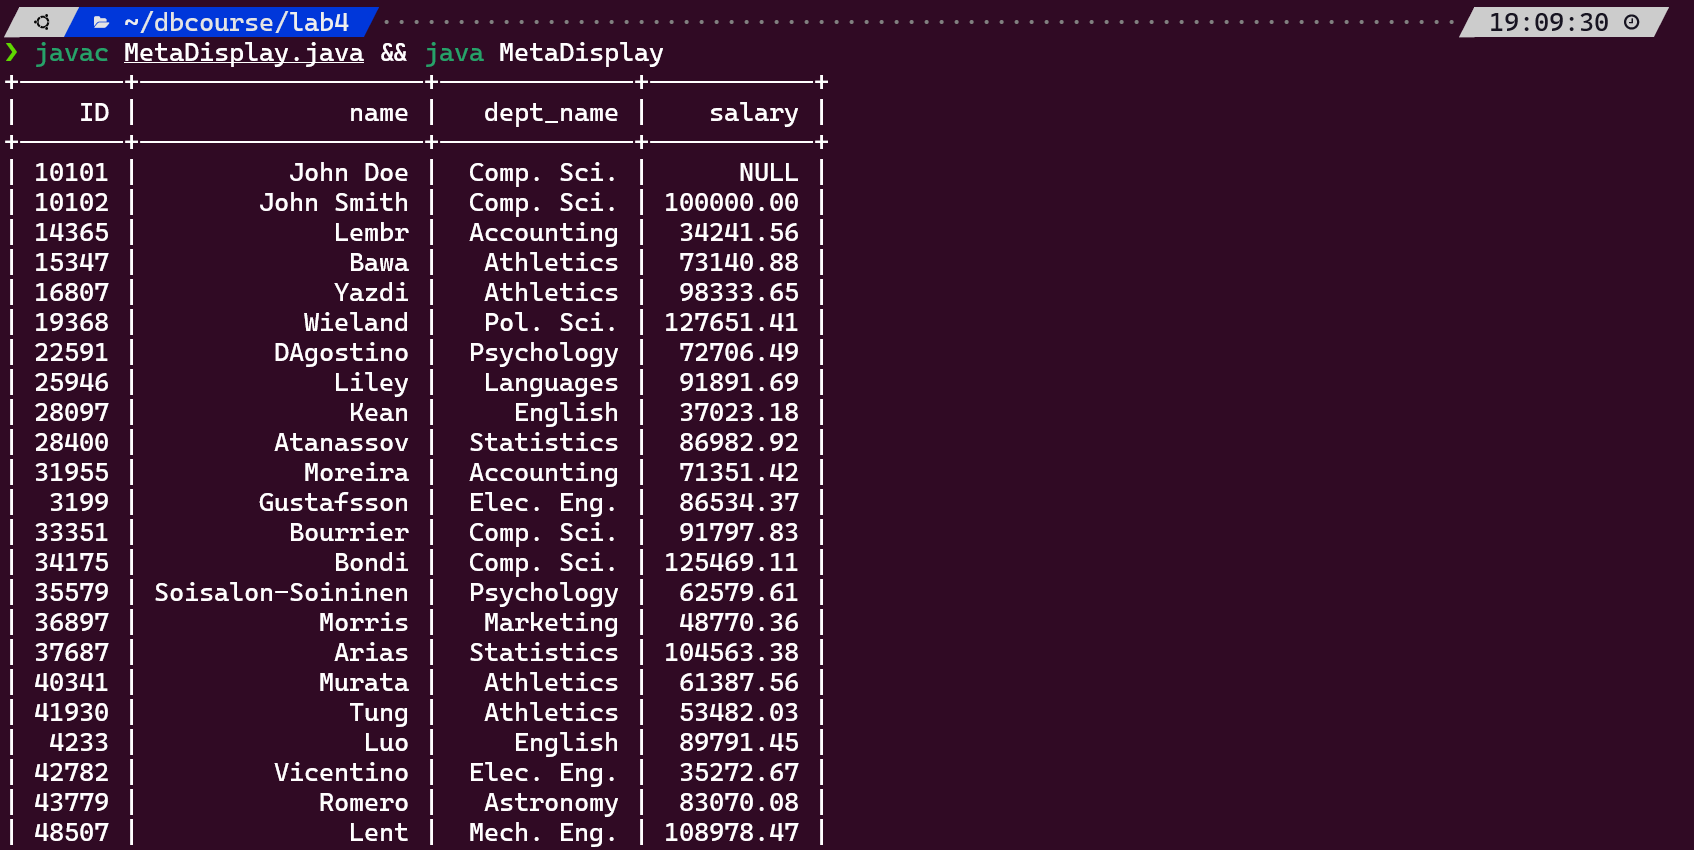
\includegraphics[width=0.9\textwidth]{img/14.png}
  \caption{MetaDisplay}
\end{figure}


\section{存在的问题及解决方案}

\begin{enumerate}
  \item 在尝试与数据库建立连接时,出现``找不到xx类''的错误,这是由于环境变量\tt{CLASSPATH}设置错误,在设置\tt{CLASSPATH}时,应该将\tt{mysql-connector-java-8.4.0.jar}的详细路径添加到\tt{CLASSPATH}中,需要精确到\tt{.jar}文件的路径,而不是目录,或者也可以使用 \tt{/*}来通配目录下的所有\tt{.jar}文件。另外,还需要注意,\tt{CLASSPATH}中还应该包含当前目录,即\tt{.},否则也会出现找不到类的错误。
  \item 运行时出现报错 \tt{java.sql.SQLNonTransientConnectionException: Public Key Retrieval is \\not allowed},这是由于新版MySQL默认不允许\tt{PublicKeyRetrieval},需要在连接URL中添加\\ \tt{allowPublicKeyRetrieval=true} 参数。
  \item 在判断 \texttt{ResultSet} 是否为空时,使用了 \texttt{if(!rs.next())},导致第一行数据丢失,可以考虑改用 \\ \texttt{if(!rs.isBeforeFirst())}。
\end{enumerate}


\section{实验小结}

通过本次实验,我学会了通过JDBC接口访问关系数据库的基本方法,掌握了JDBC的基本操作,包括与数据库建立连接、在数据库中创建数据表、向数据表中插入数据、从数据表中查询数据、更新数据表中的数据、删除数据表中的数据、使用 prepare 语句向数据表中批量插入(更新)数据、以及JDBC应用,包括Teaching Record Management System和MetaDisplay两个例子。通过本次实验,我对JDBC有了更深入的了解,掌握了JDBC的基本操作,为以后的数据库应用开发打下了基础。

\end{document}